% !TEX root = ../thesis-example.tex
%

\chapter{ARCH/GARCH Volatility Models}

\section{ARCH}

An ARCH (autoregressive conditionally heteroscedastic) model is a model for variance of time series. ARCH models are used to descirbea changing, possibly volatility varance. models were created in the context of econmetric and finance problems having to do with the amount that investments or stock increases (or decrease) per time period, so there's a tendency to descibe them as models for that type of variable. For that reason, the variable of interests will be log returns. 

\begin{figure}[!h]
	\centering
	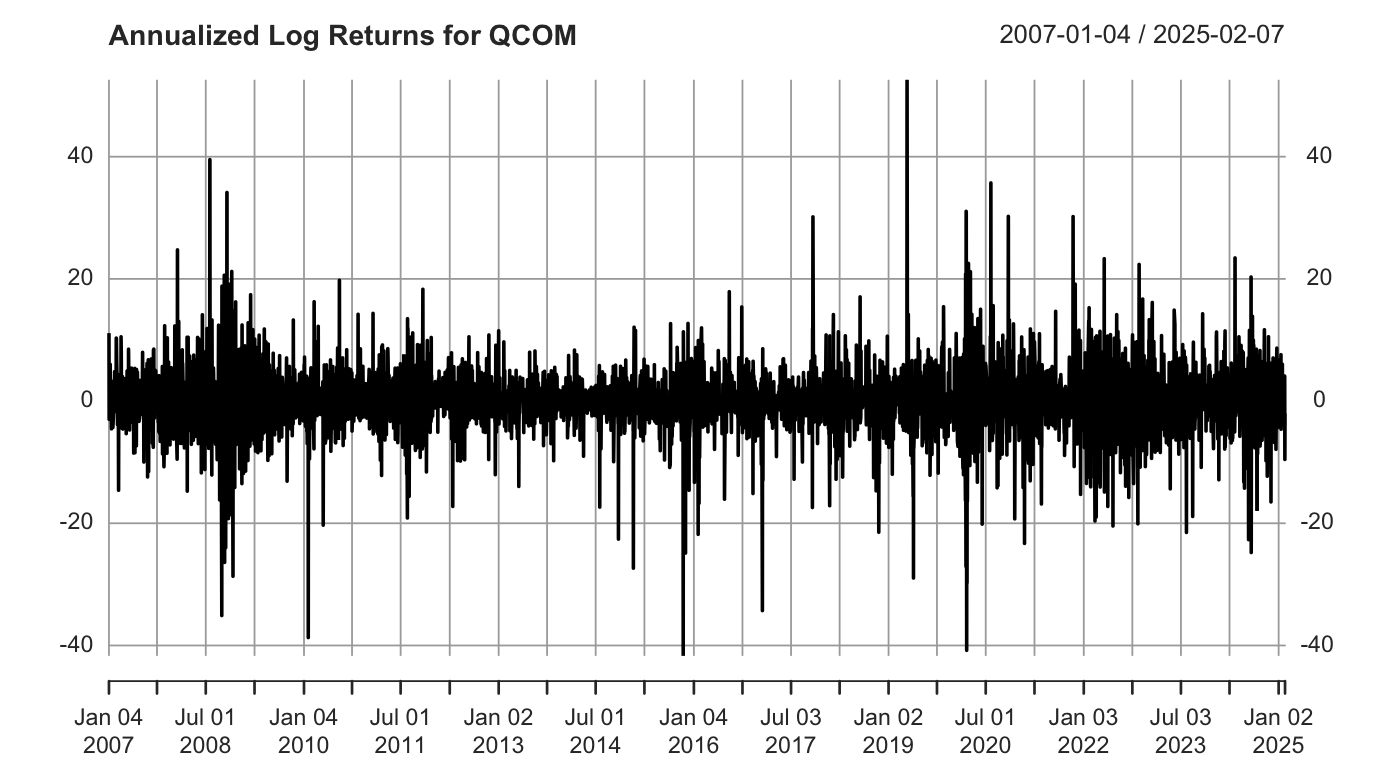
\includegraphics[width=0.8\linewidth]{content/plots/qcom_log_returns.png}
	\caption{Annaulized Logged Returns of QCOM}
	\label{fig:qcom_returns}
\end{figure}

The ARCH(1) model for the variance of model $r_t$ is that conditional on $r_{t-1}$, the variance at time $t$ is 
\begin{equation}
	\text{Var}\left(r_t|r_{r_{t-1}}\right)=\sigma_t^2=\alpha_0+\alpha_1r_{t-1}^2\quad 
\end{equation}

Figure (\ref{fig:qcom_returns}) shows the annualized log returns for QCOM  from January 4, 2007, to February 7, 2025. The returns are highly volatile, with pronounced spikes-both positive and negative-especially noticeable during periods like the 2008 financial crisis and the COVID-19 pandemic in 2020. Overall, the data oscillates around zero, reflecting frequent fluctuations in QCOM’s stock returns over the observed period. An ARCH model could be used for any series that has periods of increased or decreased variance. This might, for example, be a propery of residuals after an ARMA or ARIMA model has been fir to the data. As such, we will use the ARMA(2,2) that we have built earlier.

\begin{figure}[!h]
	\centering
	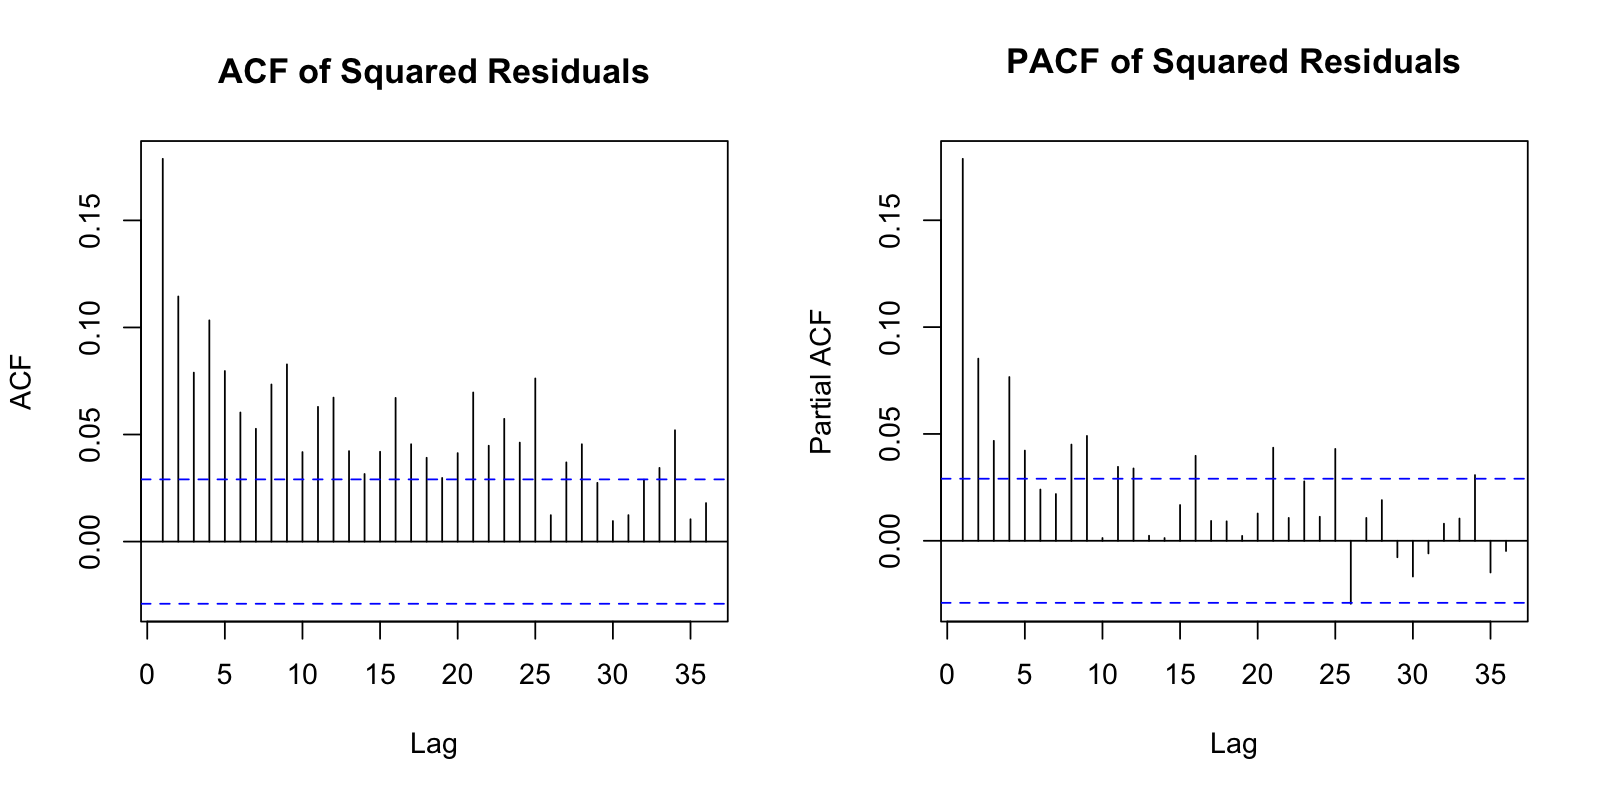
\includegraphics[width=0.85\linewidth]{content/plots/ACF_PACF_squared_residuals_QCOM.png}
	\caption{ACF and PACF of the Squared Residuals of ARMA(0,2)}
	\label{fig:ACF_PACF_residuals_QCOM}
\end{figure}

Figure (\ref{fig:ACF_PACF_residuals_QCOM}) displays the ACF/PACF in the ARMA(2,2) model residuals. For the ACF plot, we see multiple significant autocorrelations that extend well above the signficance bounds. The first several lags (particularly lags 1-5) show strong positive autocorrelation. There is also persistence of significant spikes throughout many lags that indicate strong volatility clustering. There is also a decaying pattern, which is typical of financial time series with conditional heteroskedasticity. The PACF plot of the right shows strong significant spikes at early lags, particularly from lags 1-3. There are also several additional significant lags scattered throughout the plot.

The plot provides clear evidence of the ARCH effects in QCOM. this is confirmed by the  The ARMA(0,2) model alone is not enough to capture the time-varying volatility in the QCOM time series, as there are significant autocorrelations extending across multiple lags. This suggest that higher-order ARCH model would be needed. Alternatively, we could use a GARCH-type model, which would provide more parsimonious fit given the persistent nature of the autocorrelation.

\section{GARCH}

An ARCH(m) proces is one for which the variance at time $t$ is conditional on observations at the previous $m$ times, and the relationship is

\begin{equation}
	\text{Var}\left(r_t|r_{r_{t-1},\ldots,r_{t-m}}\right)=\sigma_t^2=\alpha_0+\alpha_1r_{t-1}^2+\ldots+\alpha_{m}r_{t-m}^2
\end{equation}

With certain constraints imposted on the coefficients, the $r_t$ series squared will theortically be $AR(m)$. On the other hand, GARCH (generalized autoregressive conditionally heteroscedastic) model uses values of past squared observations and past variances to model the variances at time $t$. 

The GARCH model is an extension of the ARCH($p$) model. We notice the additional term shown above when defining the conditional variance (volatility $\sigma_t^2$ at time $t$), which allows for modeling the conditional variance to be dependent on lagged versions of itself, using a lienar combination of $\alpha_0,\alpha_1,\ldots,\alpha_n$ and the conditional variances at previous times. This addition ot the model statement makes GARCH models more flexible and able to capture the persisitence of volatility. We first start by building the GARCH(1,1) model using the mean of the ARMA(0,2) model.

\subsection{GARCH(1,1)}

\begin{figure}[!h]
	\centering
	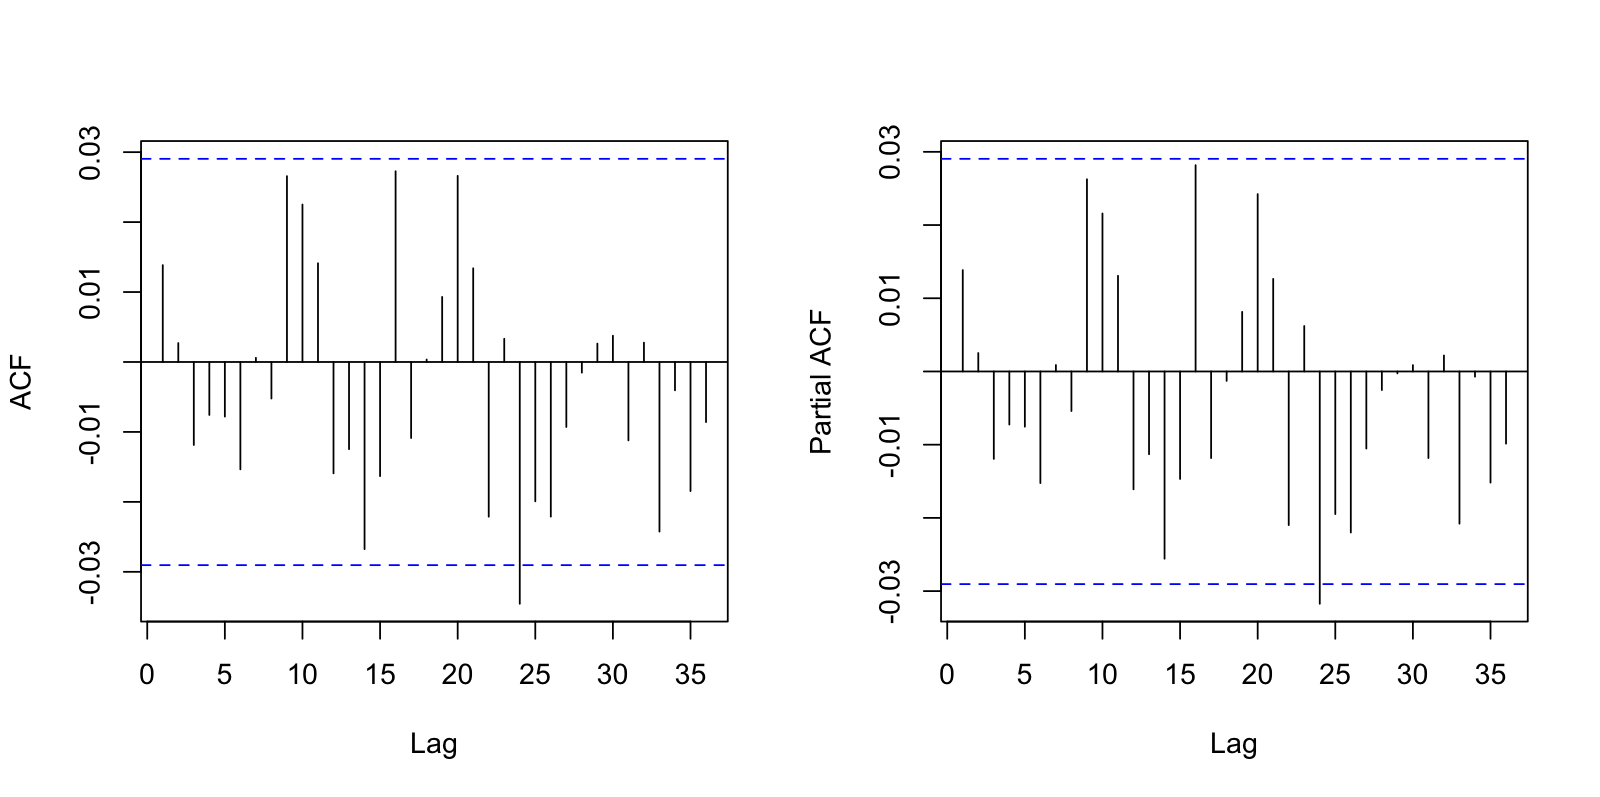
\includegraphics[width=0.85\linewidth]{content/plots/acf_pacf_std_resid.png}
	\caption{ACF and PACF of the Standard Residuals of GARCH(1,1) with ARMA(0,2) mean}
	\label{fig:acf_pacf_std_resid}
\end{figure}


Figure (\ref{fig:acf_pacf_std_resid}) shows the ACF/PACF standard residuals from GARCH(1,1) with ARMA(0,2) mean. The ACF plot shows that most autocorrelations are within the significance bounds, with only a few minor expects (lag 5). Otherwise, there are no systematic patterns of significant autocorrelation across lags. The PACF again shows a significant spike at lag 5, but all other lags fall within the confidence bounds. The lack of significant autocorrelation in both plots suggest that the ARMA(0,2) specification has adequately captured the linear dependence in the means of QCOM. The isolated spikes at lag 5 are likely due to random noise rather than model misspecification.

Figure (\ref{fig:acf_pacf_squared_resid}) shows the ACF/PACF plots for squared residuals of the GARCH(1,1) model. A notable significant spike at lag 1 that clearly exceeds the confidence bounds. We also have some other minor spikes at various lags that approach but mostly stay within the significance boundaries. In terms of the PACF, we have mutliple significant lags at 3. 

\begin{figure}[!h]
	\centering
	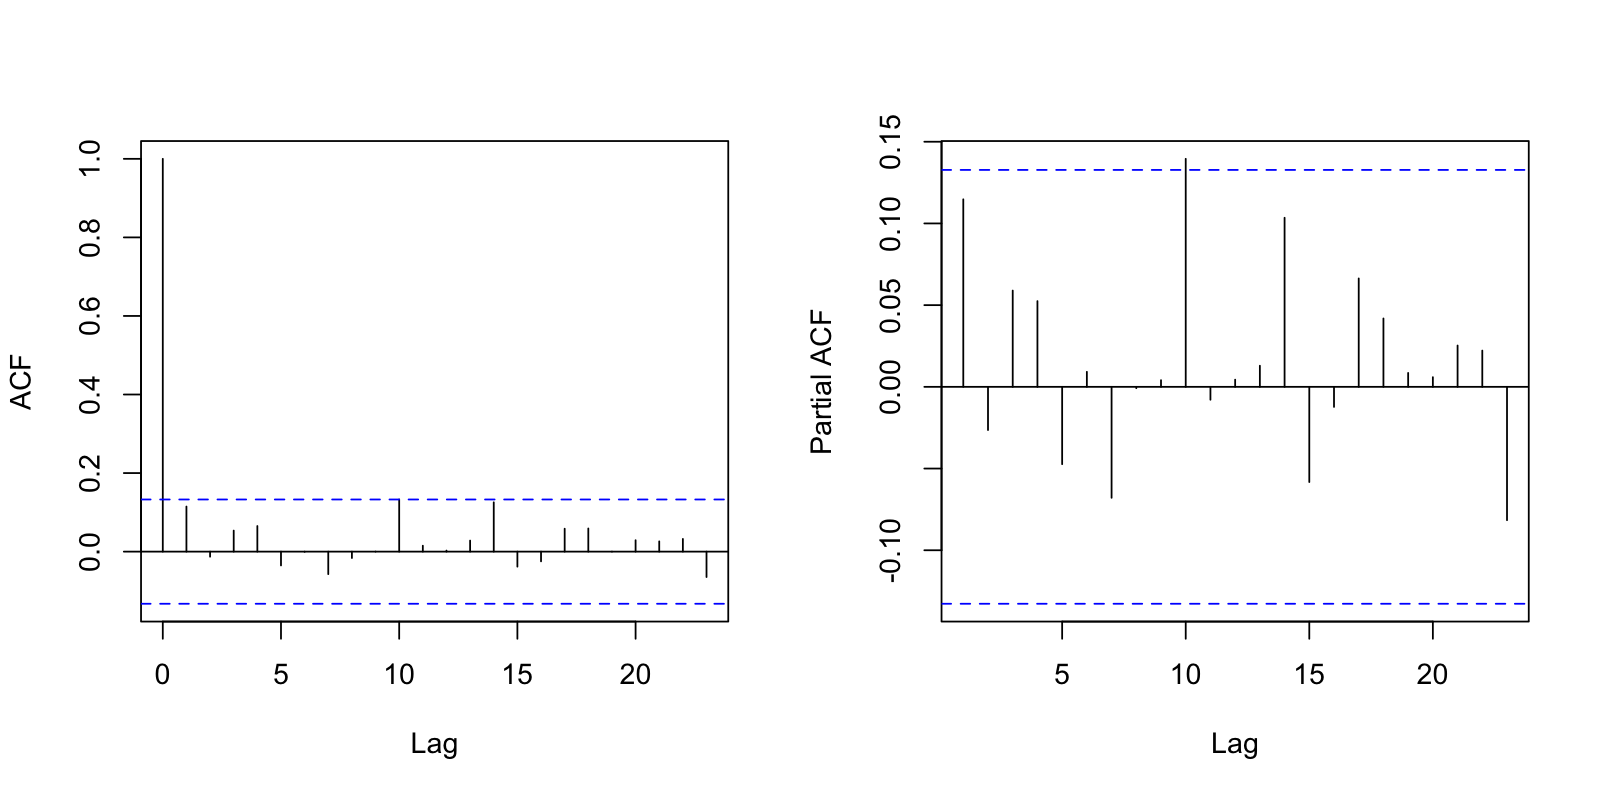
\includegraphics[width=0.85\linewidth]{content/plots/acf_pacf_squared_resid.png}
	\caption{ACF and PACF of the Squared Residuals of GARCH(1,1) with ARMA(0,2) mean}
	\label{fig:acf_pacf_squared_resid}
\end{figure}

This shows that there may be some remaining ARCH effects in the model, and more refinement is necessary.

We find the the optimal GARCH orders by using the EACF, which involves  locating the corner of insignificant autocorrelations (marked o); a similiar process for identifying the optimal ARIMA model. As we can see Table (\ref{tab:eacf_garch}) shows the first clear triangle which starts at AR=1 (GARCH Term) and MA=4 (ARCH term), suggesting a GARCH(1,1) specification, which is our first model of choice.

\begin{table}[H]
	\centering
	\caption{Extended Autocorrelation Function (EACF) for QCOM Log Returns}
	\begin{tabular}{c|cccccccccccccc}
		$(p, q)$ & 0 & 1 & 2 & 3 & 4 & 5 & 6 & 7 & 8 & 9 & 10 & 11 & 12 & 13 \\
		\hline
0 & o & o & o & o & o & o & o & o & o & o & o & o & o & o \\
1 & x & o & o & o & o & o & o & o & o & o & o & o & o & o \\
2 & x & x & o & o & o & o & o & o & o & o & o & o & o & o \\
3 & x & x & x & o & o & o & o & o & o & x & o & o & o & o \\
4 & x & x & x & x & o & o & o & o & o & o & o & o & o & o \\
5 & x & x & x & x & o & o & o & o & o & o & o & o & o & o \\
6 & x & x & x & o & x & o & o & o & o & o & o & o & o & o \\
7 & o & o & x & o & x & o & o & o & o & o & o & o & o & o \\
		\label{tab:eacf_garch}
	\end{tabular}
\end{table}

\section{Forecasting}

An ARMA(2,2)-GARCH(1,1) model combines an Autoregressive Moving Average (ARMA) model for the conditional mean of a time series with a Generalized Autoregressive Conditional Heteroskedasticity (GARCH) model for its conditional variance. The mathematical derivation for the ARMA(2,2)

\begin{equation}
\begin{aligned}
	r_t &= \mu + \phi_1 r_{t-1} + \phi_2 r_{t-2} + \theta_1 \epsilon_{t-1} + \theta_2 \epsilon_{t-2} + \epsilon_t \\
	&= 1.74405 - 0.05736\, r_{t-1} + 0.87125\, r_{t-2} - 0.11683\, \epsilon_{t-1} - 0.98070\, \epsilon_{t-2} + \epsilon_t
\end{aligned}
\end{equation}
where $r_t$ is the value of the time series at time $t$, $\mu$ is the constant term, $\phi_1$ and $\phi_2$ are the autoregressive coefficients for the first and seceond lags of $r_t$, $\theta_1$ and $\theta_2$ are the moving average coefficients for the first and second lags of the error term $\epsilon_t$

\begin{equation}
	\begin{aligned}
		\sigma_t^2 &= \omega + \alpha_1 \epsilon_{t-1}^2 + \beta_1 \sigma_{t-1}^2 \\
		&= 31.9997 + 0.04625\, \epsilon_{t-1}^2 + 0.89064\, \sigma_{t-1}^2
	\end{aligned}
\end{equation}
where $\sigma_t^2$ is the conditional variance at time $t$, $\omega$ is the constant term in the variance equation, $\alpha_1$ is the ARCH parameter, which measures the reaction to conditional variance to past shocks, and $\beta_1$ is the GARCH parameter, which measures the persistence of the conditional variance based on past conditional variances. 

The term $\omega $ term (32.000), representing a baseline variance, is not statistically significant ($p$=0.118). The `alpha1` coefficient (0.046), which captures the impact of past shocks on volatility, is also not statistically significant (p=0.137), suggesting a weak immediate reaction of volatility to new information. However, the `beta1` coefficient (0.891) is highly significant (p=0.000) and close to 1, indicating strong persistence in volatility; past volatility levels are a key determinant of current volatility, causing volatility clustering. The sum of $\alpha_1 $and $\beta_1$ (0.046 + 0.891 = 0.937) is high, confirming that shocks to volatility are quite persistent, though the sum being less than 1 implies the variance process is stationary.

\begin{figure}[!h]
	\centering
	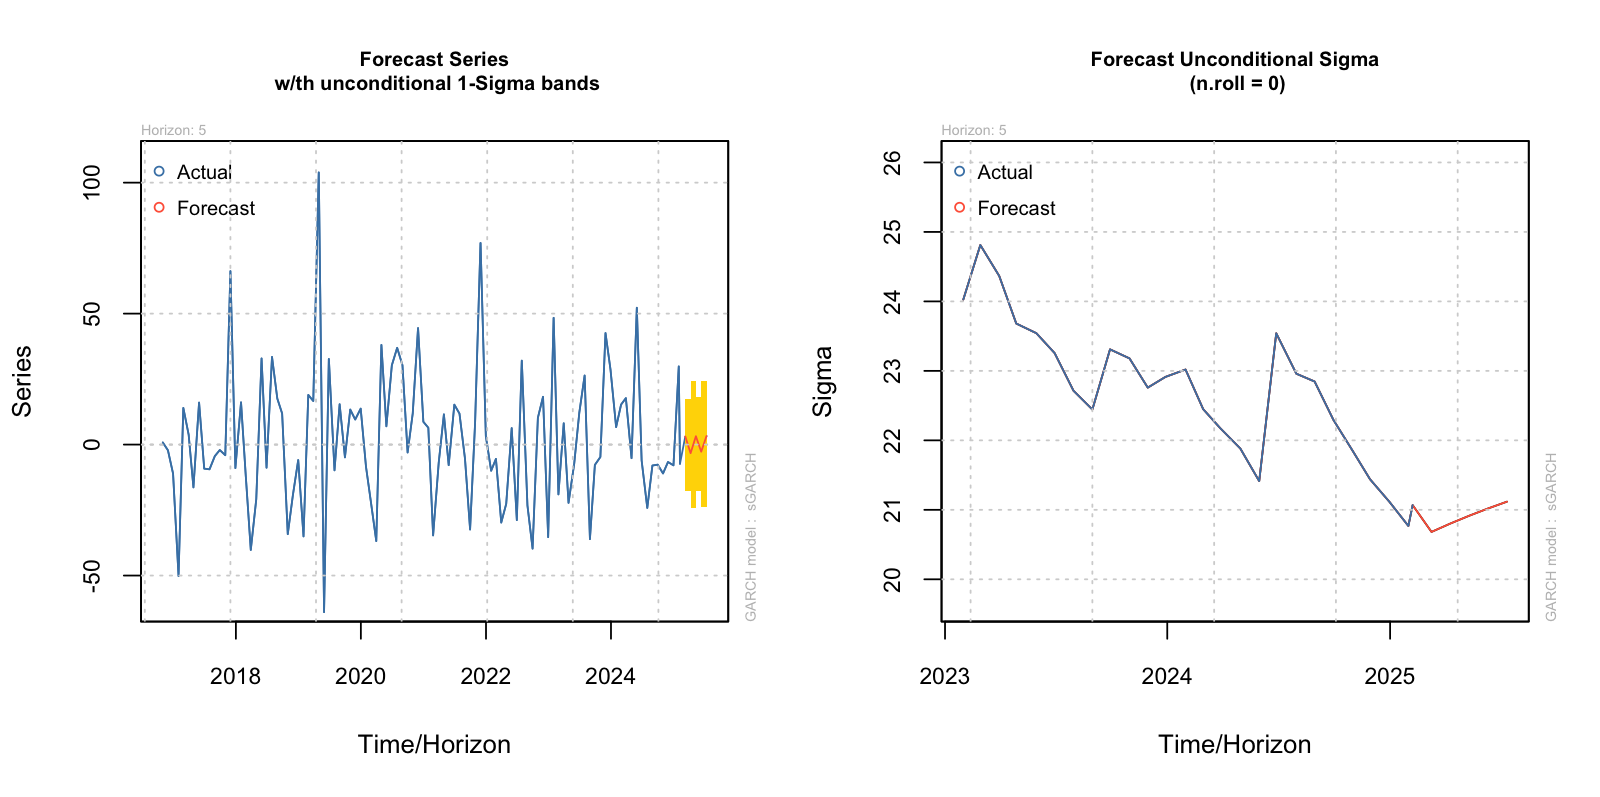
\includegraphics[width=0.85\linewidth]{content/plots/GARCH_forecast.png}
	\caption{ACF and PACF of the Squared Residuals of GARCH(1,1) with ARMA(0,2) mean}
	\label{fig:GARCH_forecast}
\end{figure}

Figure (\ref{fig:GARCH_forecast}) shows the forecast for the GARCH(1,1) model with ARMA(2,2) mean, which provides valuable insights into both the predicted returns and volatility patterns. The left panel displays the historical series (blue line) characterized by significant fluctuations over the 2018-2025 period, with several dramatic spikes exceeding 50 units in both positive and negative directions. The forward-looking forecast (orange line) projects relatively modest returns with a slight upward trend, accompanied by widening yellow confidence bands that reflect increasing uncertainty over the 5-period forecast horizon. This suggests that while the model anticipates positive returns in the near future, it acknowledges considerable uncertainty in these predictions, consistent with the historical volatility observed in the series.


The right panel, displaying unconditional sigma (volatility) forecasts, reveals that volatility has followed a generally declining trend from about 24.5 units in early 2023 to approximately 20.7 units by early 2025. The model forecasts a modest uptick in volatility over the next five periods. This slight increase in projected volatility aligns with the expanding confidence intervals seen in the returns forecast. The overall pattern suggests that while the GARCH model expects volatility to remain lower than historical peaks, it anticipates some volatility persistence - a typical characteristic of financial time series modeled with GARCH specifications. This measured increase in forecasted volatility indicates the model’s response to recent market conditions, though the magnitude remains relatively contained compared to historical levels.

